\chapter{The LHC and CMS experiment}

%\clearpage
\section{The LHC}

The Large Hadron Collider (LHC) is the largest and most powerful particle accelerator in the world. The LHC was installed in an existing 26.7 km tunnel that was constructed for the LEP machine between 1984 and 1989. The LHC tunnel has 8 straight sections and 8 arcs, and is located between 45m and 170m below the surface. The LHC hosts 4 experiments currently: CMS (Point 5), ATLAS (Point 1), ALICE (Point 2) and LHCb (Point 8). The LHC can accelerate the proton beam to 7 TeV (running at 6.5 TeV during the LHC Run 2, the data used for this thesis).

However, the LHC is not the only CERN accelerator needed to boost the proton to such a high energy. The LHC is the last and biggest accelerator in the chain. A simplified injection chain is shown in Fig~\ref{fig:c3lhclpsspslhc}. Hydrogen gas is injected into a metal cylinder, and then placed in a strong electrical field to strip the electron from hydrogen to obtain bare protons. The protons are accelerated to 90 keV with a DC voltage power supply. Then a Radio Frequency Quadrupole (QRF) focuses and boosts the protons to 750 keV. After that, the proton beam is injected into a linear accelerator (LINAC2) and accelerated to 50 MeV. The LINAC2 will be replaced by the LINAC4 with a negative hydrogen ion source (H$^{-}$), and a higher beam intensity and energy (160 MeV) in 2019-2020. 

\begin{figure}[htbp]
 \begin{center}
  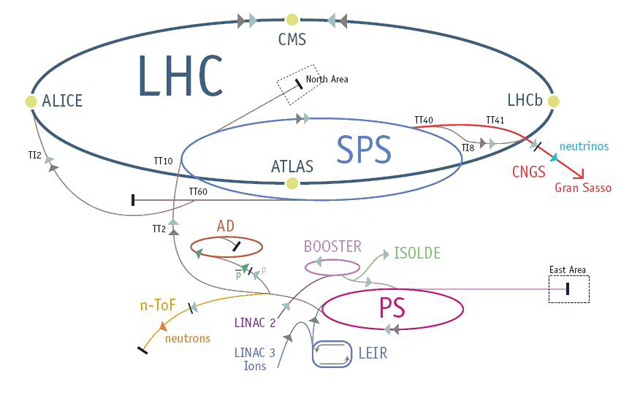
\includegraphics[width=0.8\textwidth]{figures/c3/c3_lhc_lpsspslhc.jpg}
 \end{center}
 \caption{The LHC full injection chain.}
 \label{fig:c3lhclpsspslhc}
\end{figure}

The proton beam is boosted to 6.5 TeV with four circular accelerators from the linear accelerator. The first one in the chain is the proton synchrotron booster (PSB, Fig~\ref{fig:c3lhcpsb}), a four-ring slow-cycling synchrotron. The PSB was inserted in between the LINAC and proton synchrotron in 1972 to increase the beam intensity. The PSB increases the proton energy up to 1.4 GeV in 530 ms and then injects the beam into the proton synchrotron (PS). The protons are accelerated to 25 GeV inside the PS. The super proton synchrotron (SPS) takes the beam from the PS and boosts it to 450 GeV in 4.3 seconds. And finally, the protons are injected into the LHC and are accelerated up to 6.5 TeV in 25 minutes during so-called beam ramp-up. 

\begin{figure}[htbp]
 \begin{center}
  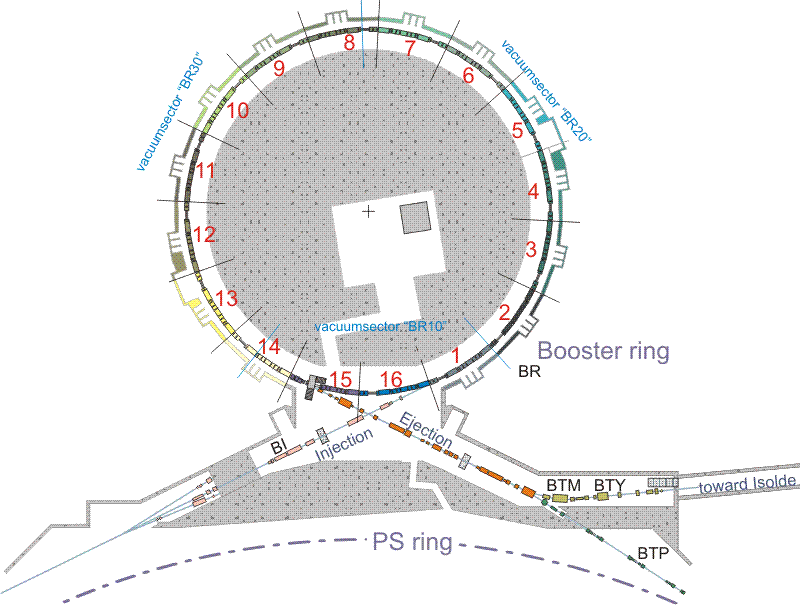
\includegraphics[width=0.8\textwidth]{figures/c3/c3_lhc_psb.png}
 \end{center}
 \caption{The PS layout.}
 \label{fig:c3lhcpsb}
\end{figure}

We can perform a simple calculation to estimate how long it takes protons to travel from the LINAC2 until they have 450 GeV of energy in the SPS: 0.53+1.025+4.3=5.86 seconds. However, we also split one fill of the beam into several bunches and batches with certain time spacing to obtain a desired luminosity. Therefore, we have latency for different batch and the 5.86 seconds is just a lower limit for pre-LHC acceleration time. 

%The fill scheme before the LHC is relatively stable in the machine in the proton physics mode. The injection beam from the PSB to the PS contains 2 batches, 4 bunches for the first batch and 2 for the second. The first takes an additional 1200ms to be delivered. The proton beam will go through one triple split and two double splits. A 72 bunches beam will be formed after the splitting and delivered to SPS in a group of 4 72-bunch batches. The latencies are 10.8 seconds for the first batch, 7.2 for the second, 3.6 for the third and 0 for the fourth. Therefore, the maximum time from the LINAC2 to 450 GeV SPS is 0.53+1.2+1.025+10.8+4.3=17.86 seconds. 

The LHC fill scheme can be different for various purposes. A common fill scheme has 2808 bunches in the LHC ring. This fill scheme is illustrated in the Fig~\ref{fig:c3lhcfillscheme}. The SPS will have 12 injections to the LHC. The number of 72-bunch batches are in the pattern of 234 334 334 334. There are different luminosities for different fill schemes. In the detector operation, it is important to know the fill scheme and expected luminosity in advance to in order to design the trigger menu. 

\begin{figure}[htbp]
 \begin{center}
  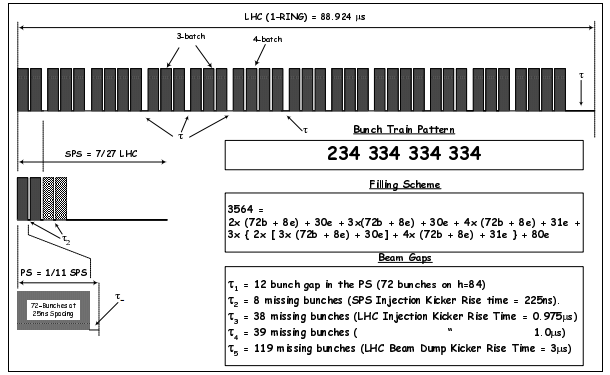
\includegraphics[width=0.8\textwidth]{figures/c3/c3_lhc_fillscheme.png}
 \end{center}
 \caption{Schematic of the Bunch Disposition around an LHC Ring for the 25 ns Filling Scheme.}
 \label{fig:c3lhcfillscheme}
\end{figure}

%\clearpage
\subsection{LHC: Machine layout and performance}

The LHC is a nearly circular ring with 8 arcs and 8 straight sections (Fig~\ref{fig:c3lhclayout}). Each straight section is around 528 meters long and can host a detector system or infrastructure related to the accelerator. Two general purpose experiments are located at opposite straight sections: ATLAS experiment at point 1 and CMS experiment at point 5. The ALICE experiment and the clockwise circulating beam (beam1) injection system are located at point 2, while the LHCb experiment and the counter clockwise circulating beam (beam2) injection system are at point 8. 

\begin{figure}[htbp]
 \begin{center}
  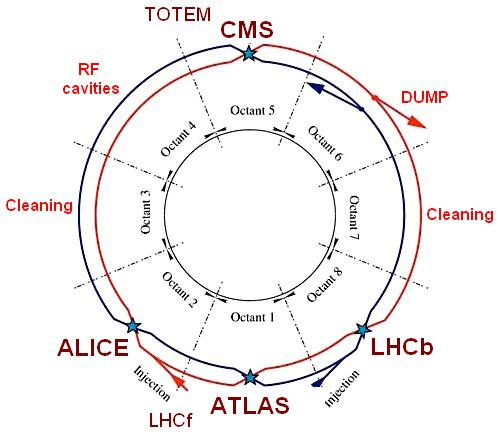
\includegraphics[width=0.8\textwidth]{figures/c3/c3_lhc_latticelayout.jpg}
 \end{center}
 \caption{The LHC layout.}
 \label{fig:c3lhclayout}
\end{figure}

Collimation systems~\cite{Assmann:691766} are located at points 3 and 7. The collimation system protects the machine against unavoidable regular or irregular beam loss. The collimator at point 3 is designed to clean beam transverse momentum dispersion and the one at point 7 is for beam betatron emission. The materials of the collimators are required to be extremely radiation hard because they are installed in the most active regions of the LHC. 

The beam dump insertion is sits at the point 6. There are three steps to dump the beam: extraction, dilution and absorption. The magnet kicker can be turned on in 3000 ns, which is the time interval required for each beam to orbit around the LHC ring. Then the beam is deflected at an angle of 0.27 mrad. The extracted beam is swept in a quasi-circular orbit by two sets of deflecting dilution kickers. Finally, a 7m long segmented carbon cylinder absorbs the beam.

Point 4 is the only straight section that contains acceleration systems. Two radio frequency systems are installed for both beam1 and beam2. 

One of the main aims of the LHC is to detect physics beyond the standard model. The study of the rare events in the LHC requires both high beam energies and high beam intensities. The energy of the beam is limited by the machine geometry. The luminosity of the machine can be described by Eq~\ref{eq:c3lhclumi} with the Gaussian beam distribution. The $N_{b}$ term is the number of particles per bunch and $n_{b}$ is the number of bunches per beam. This indicates that we can increase the luminosity through optimization of the fill scheme. The $f_{rev}$ term is the revolution frequency, $\gamma_{r}$ is the relativistic gamma factor, $\varepsilon_{n}$ is the normalized beam emittance and $\beta *$ is the impact parameter at the collision point. The F term is the geometric luminosity reduction factor due to the crossing angle at the interaction point. 

\begin{equation}
 L = \frac{N^{2}_{b}n_{b}f_{rev}\gamma_{r}}{4\pi \varepsilon_{n}\beta *}F \;
 \label{eq:c3lhclumi}
\end{equation}

The definition of F is given in Eq~\ref{eq:c3lhcgeof}. The $\theta_{c}$ term is the full crossing angle at the interaction point, the $\sigma_{z}$ is the RMS bunch length and $\sigma *$ is the transverse RMS beam size at the interaction point. The LHC experts are trying to reduce the crossing angle from 370 to 280 mrad, which will increase the peak luminosity by 15 \%. 
\begin{equation}
 F = (1+\frac{\theta_{c}\sigma_{z}}{2\sigma *})^{-1/2} \;
 \label{eq:c3lhcgeof}
\end{equation}

In the CMS and ATLAS experiments, the design peak luminosity at the collision point is approximately 10$^{34}$cm$^{-2}$s$^{-1}$. The LHC achieved this goal in 2016. Attempts are now being made to increase to increase the luminosity through further optimization.

%\clearpage
\subsection{LHC: From an operational point of view}

The LHC is an extremely complex machine and it is almost impossible to grasp every detail. However, the LHC provides a summary of status for its operational activities, which are very useful in for detector operation.

\subsubsection{Accelerator mode}

The accelerator mode indicator provides a summary of the status of the LHC machine. All the accelerator modes are listed in Table~\ref{tab:c3lhcaccmode}. The accelerator modes can be divided into two groups by the presence or not of the beam. For example, ACCESS mode means that the LHC group or at least one of the detector system groups needs access to the machine area, with the beams off, to investigate a problem. The beam must be dumped or already be off to allow this access period. Another example is the BEAM SETUP mode, which means the beam is under preparation. The beam modes are described in the following section. The detector systems (e.g., CMS) make daily operational decisions depending on the accelerator modes and beam modes provided by the LHC.

\begin{table}[htbp]
\fontsize{10 pt}{1.2 em}
\selectfont
\begin{centering}
\caption{\label{tab:c3lhcaccmode} Accelerator Mode.}
\hspace*{-4ex}
\begin{tabular}{|c|c|c|}
\hline
 Mode Name &  Description & Beam exist \\
\hline
 SHUTDOWN & \specialcell{Machine not running} & NO BEAM \\
\hline
 COOLDOWN & \specialcell{Machine comes back from shutdown,\\ cryogenics related activities going on} & NO BEAM \\
\hline
 MACHINE CHECKOUT & \specialcell{Checking out LHC subsystems} & NO BEAM \\
\hline
 ACCESS & \specialcell{Access going on} & NO BEAM \\
\hline
 MACHINE TEST & \specialcell{Operation tests without beam} & NO BEAM \\
\hline
 CALIBRATION & \specialcell{Power converter calibration} & NO BEAM \\
\hline
 WARM-UP & \specialcell{Sectors warm up for repair} & NO BEAM \\
\hline
 RECOVERY & \specialcell{Quench recovery} & NO BEAM \\
\hline
 SECTOR DEPENDENT & \specialcell{Sector activities going on} & NO BEAM \\
\hline
 BEAM SETUP & \specialcell{Machine setup with 1 or 2 beams,\\ usually a signal of next \\ physics fill when taking data} & BEAM \\
\hline
 PROTON PHYSICS & \specialcell{Beam on for proton physics} & BEAM \\
\hline
 ION PHYSICS & \specialcell{Beam on for ion physics} & BEAM \\
\hline
 TOTEM PHYSICS & \specialcell{Beam on for TOTEM physics} & BEAM \\
\hline
 MACHINE DEVELOPMETN & \specialcell{Beam on machine development} & BEAM \\
\hline
\end{tabular}
\par\end{centering}
\end{table}

\subsubsection{Beam mode}
The beam modes are shown in the Table~\ref{tab:c3lhcbeammode}. The beam modes describe standard injection procedures and accidental abort issues of the two beams in the LHC. A standard successful injection for physics should have the following beam modes in sequence during the BEAM SETUP accelerator mode:

\begin{itemize}
\item BEAM SETUP: The SPS is injecting beam bunches into the transfer line. The beam is not circulating yet in the LHC.
\item INJECTION PROBE BEAM: A test beam with relatively small intensity is being injected into the LHC from the transfer line. Although we have a machine protection system to shield the LHC from the beam, we still need to make sure the system is safe for beam circulation.
\item INJECTION SETUP BEAM and INJECTION PHYSICS BEAM: The LHC is measuring the beam properties. Then a full intensity beam will be injected for physics data taking.
\item PRERAMP and RAMP: The LHC is ramping up the beam energy up with the radio frequency system.
\item FLAT TOP and SQUEEZE: The LHC is checking the system. Then the beam will be focused to reduce the impact parameter.
\item ADJUST and STABLE BEAM: The LHC is adjusting the beams before collision. Then we can begin to enjoy the data run.
\end{itemize}

\begin{table}[htbp]
\fontsize{10 pt}{1.2 em}
\selectfont
\begin{centering}
\caption{\label{tab:c3lhcbeammode} Beam Mode.}
\hspace*{-4ex}
\begin{tabular}{|c|c|c|}
\hline
 Mode Name &  Description \\
\hline
 SETUP & \specialcell{Beam in transfer line, but not in the ring} \\
\hline
 ABORT & \specialcell{Recovery mode following beam drop} \\
\hline
 INJECTION PROBE BEAM & \specialcell{Ring is injected with test beam for safe circulating} \\
\hline
 INJECTION SETUP BEAM & \specialcell{Beam measurement going on after probe beam\\ but before injection physics beam} \\
\hline
 INJECTION PHYSICS BEAM & \specialcell{Beam for physics is injected in the ring} \\
\hline
 PRERAMP & \specialcell{Injection done, prepare for ramp} \\
\hline
 RAMP & \specialcell{Ramp up the beam energy} \\
\hline
 FLAT TOP & \specialcell{Ramp done, pre-squeeze checks} \\
\hline
 SQUEEZE & \specialcell{Squeezing the beam size} \\
\hline
 ADJUST & \specialcell{Preparing for collision or after collision} \\
\hline
 STABLE BEAMS & \specialcell{Stable collision, detector should taking data} \\
\hline
 UNSTABLE BEAMS & \specialcell{Unstable beam because of sudden beam degradation} \\
\hline
 BEAM DUMP WARNING & \specialcell{Beam dump warning in case of emergency beam dump} \\
\hline
 BEAM DUMP & \specialcell{End of physics collision} \\
\hline
 RAMP DOWN & \specialcell{Ramp down beam energy after programmed dump} \\
\hline
 CYCLING & \specialcell{Pre-cycle before injection\\ following access, recovery, etc} \\
\hline
 NO BEAM  & \specialcell{No beams exist} \\
\hline
\end{tabular}
\par\end{centering}
\end{table}

The beam modes are used to estimate the time remaining before the beginning of the subsequent data run. For example, CMS requires all the subsystem to be ready for data taking when the LHC declares injection physics beam. Some of the subsystems need to do the alignment or calibration during this period. The time estimates allowed through use of the LHC beam status is important for smooth data taking.

%\clearpage
\section{The CMS experiment}

The CMS Experiment is a particle physics experiment at the LHC. It consists of the CMS detector system and event reconstruction, supported by the detector operation team, the computing/data storage team and , the software and event reconstruction team, the detector performance groups (DPGs), the physics objects groups (POGs), the physics analysis groups (PAGs), the Publications Committee, the Conference Committee, the Authorship Committee, the spokesperson and deputies, and many other people.  In total, there are around 2500 individuals listed on a typical physics publication, and around 1000 more who contribute to the operation of the experiment.

%\clearpage
\subsection{CMS detector system}

The Compact Muon Solenoid (CMS) is one of the two general purpose detectors at the LHC, along with the ATLAS detector. To fulfill its ``general purpose", CMS is designed as a combination of several subsystems: Silicon Pixels and Strips for tracking information, Electromagnetic and Hadron Calorimeters for ``light" particle energy deposition and drift tubes and cathode strip/resistive plate chambers for muon detection. The locations of these subdectors in the CMS are not random: The silicon tracking subsystems are closest to the collision point. The calorimeters come after the silicon subdetectors, because the calorimeter absorbs all SM particles except for muons and neutrinos. Finally the muon system is the outermost detector. To obtain high performance, CMS is immersed in a 4-T magnetic field, which is provided by a super-conducting solenoid (``S" in CMS). The magnet contributes a large fraction of the CMS total weight: 12500 tons out of 14000. However, compared with its heavy weight, the size of the CMS is relatively small: only 5000 m$^{3}$. In comparison, the ATLAS detector weighs 7000 tons and encompasses a volume of 22500 m$^{3}$. This explains the name ``Compact" placed in front of ``Muon Solenoid" since its density is nearly to 3000 kg/m$^{3}$.

\subsubsection{Inner tracking system}

As indicated by its name --- inner tracking system, there are two main characteristics of this CMS sub-detector: it is the closest sub-detector to the LHC beam and its purpose is to reconstruct the trajectories of charged particles (``tracks") that traverse it. The main challenge is a consequence of the first feature: the inner tracking systems have to be radiation hard so that they can survive over years of operation in the intense radiation environment near the beam lines. Moreover, since the LHC has high intensity and a small time interval between bunch crossings (25 nano seconds), we also need the inner tracking systems to have a fine granularity and fast response. The silicon based technology detector is the best option to satisfy these requirements. On the other hand, the second feature actually comes from the physics requirement. We need to reconstruct the tracks of charged particles and secondary vertices in the event from the three dimensional hits. The track information is not only used in the charged particle reconstruction, but also applied in the particle flow algorithm~\cite{CMS-PAS-PFT-09-001} as a basis of all physics object reconstruction in CMS. The secondary vertices are also important in the heavy flavor object reconstruction, and in new-physics search of long-lived particles. 

As a result of budget-performance balance, the CMS inner tracking systems are designed as a combination of two sub-systems: the silicon pixel detector and the silicon strip detector. A schematic drawing of the CMS tracking system is shown in Fig~\ref{fig:c3cms2dtracker}. More details are given in the following sections. 

\begin{figure}[htbp]
 \begin{center}
  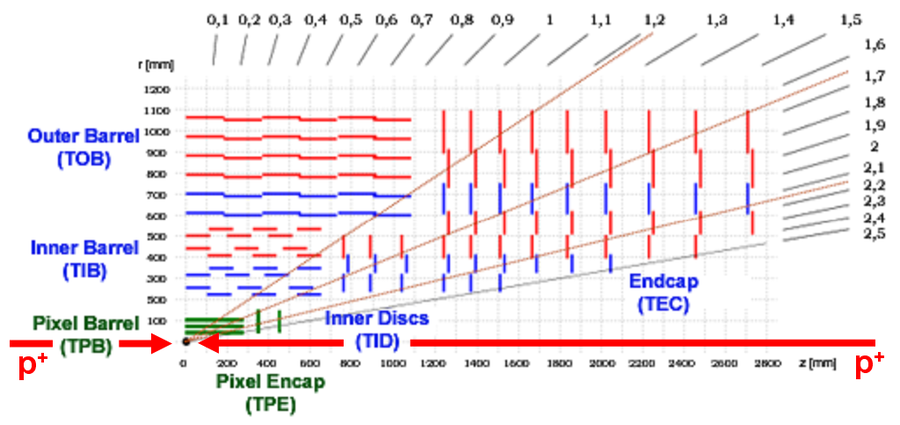
\includegraphics[width=0.8\textwidth]{figures/c3/c3_cms_2dtracker.png}
 \end{center}
 \caption{Two dimensional CMS inner tracking system layout, phase 0.}
 \label{fig:c3cms2dtracker}
\end{figure}

\paragraph{Silicon pixels}
The pixel system is the part of inner tracking system that is closest to the collision point. It provides a precise measurement of the tracking and therefore makes a major contribution to the secondary vertex reconstruction. The pixel cells are distributed with a size of 100 $\mu m$ $\times$ 150 $\mu m$ in three-dimensional space, which allows a 3D reconstruction method for the secondary vertex. The signals are read by sensors and packed by readout chip. Then the signal is delivered to the front-end driver through the analog chain once a positive bit is received from the L1 trigger.

The CMS detector system has three phases, corresponding to different stages of the LHC. Phase 0 CMS is the baseline detectors for the LHC with 7 or 8 TeV and integrated luminosity around 25 fb$^{-1}$. Phase 1 CMS is the first detector upgrades for 13 or 14 TeV and integrated luminosity around 300 fb$^{-1}$. Phase 2 CMS is the major upgrade for high-lumi LHC (HL-LHC) with 3000 fb$^{-1}$. The phase 0 pixel detector contains three barrel layers (BPix) and two endcap disks (FPix), which cover a pseudorapidity range $-2.5<\eta<2.5$. The pseudorapidity $\eta$ is a spatial coordinate describing the angle angle of a particle relative to beam axis. It is defined as $\eta = -ln[tan(\frac{\theta}{2})]$, where $\theta$ is the angle between the particle three-momentum and beam direction. In the phase 1 upgrade~\cite{Klein:2140071}, because of radiation damage, all layers and disks were replaced with new ones, and an additional layer was added both in the barrel region and in both endcap regions.

%One special design of the pixel detector is the blade that module mounted are rotated by 20 degrees in a turbine geometry. Such an arrangement enhanced the charge sharing effects~\cite{Giurgiu:2008ir} between the nearby pixels. The space resolution can be improved to 15 $\mu m$ by the using the ``charge sharing" effect in pixels. CMS take advantage of this effect with the analog readout of the collected charges by readout pixels in-group with readout chips. 

\paragraph{Silicon strips}

The particles pass through ten layers of silicon strip detectors after the pixels. The silicon strip tracker is composed of 15148 detector modules. Each module is composed of either one 320 $\mu m$ or two 500 $\mu m$ silicon sensors from a total of 24244 sensors. The signal from a sensor is amplified, shaped and stored by a custom integrated circuit. Once a positive L1 trigger decision is received, the analog signal is multiplexed and transmitted via an optical link to the front end driver, then digitalized. 

The inner strip detector contains 4 barrel layers (TIB) and 3 endcap disks (TID) on each side. The outer strip detector has 6 barrel layers (TOB, 2 double-sided, 4 single-sided) and the endcap strip has 9 disks (TEC) on each side.

A laser alignment system~\cite{Sirunyan:2017rbc} is used to monitor the stability and the alignment of the strip detector mechanical structure. An infrared laser light is delivered directly to the sensor on the 434 silicon modules (3\%) to trigger a signal pulse. The alignment data can be taken during commissioning, an inter-fill period or in the orbit gap with stable beams. The pixel detector is aligned with strip detector using the reconstructed tracks, and therefore the strip alignment is the only online and direct alignment needed for the inner tracking system. 

\subsubsection{Calorimeters}

\paragraph{Electromagnetic calorimeter}
The CMS electromagnetic calorimeter (ECAL) is a hermetic homogeneous calorimeter made of lead tungstate ($PbWO_{4}$) crystals. Lead tungstate is an appropriate choice for the ECAL because the crystal is both radiation hard and has a rapid response (same level as the LHC bunch crossing). In total 61200 lead tungstate crystals are installed in the ECAL barrel region while 7324 are installed in each endcap. Lead tungstate emits 80\% of the light in 25 ns once an electron (or photon) strikes on the crystal.

A photon detector is needed to collect the light yield from the crystals. As for the crystal, the photon detector needs to be both radiation tolerant and fast. To satisfy these requirements, avalanche photodiodes (APD) are installed in barrel and the vacuum phototriodes in the endcap. All the photon detectors have been tested in a harsh environment (high radiation plus 4T magnetic field) before actually being installed. The light yield from the crystal is weak, so it needs to be amplified with a photomultiplier. Multi-gain pre-amplifiers (MGPA), and an ASIC (Application-specific integrated circuit) specifically designed for ECAL, are installed to reshape and amplify the signal from photon detectors.

The amplified signals are integrated and digitized by on-detector front end electronics and then sent to the central data acquisition system from the off-detector back end electronics. The ECAL electronics, especially for the off-detector electronics, are very similar to the phase 0 HCAL off-detector electronics. The HCAL electronics are discussed in the next section.

A last component of ECAL is the preshower system. The two photons from neutral pion decay are almost collinear when the pion energy is high. The main purpose of the preshower detector is to trigger an electromagnetic shower with high spatial resolution before the ECAL endcap. As a result, the almost collinear photons can be distinguished by the ECAL reconstruction algorithm. 

\paragraph{Hadron calorimeter}

The CMS HCAL is a set of detectors that measure the energy of hadronic particles, i.e., particles composed of quarks and gluons. It contains four parts: Hadron Barrel (HB), Hadron Endcap (HE), Hadron Outer (HO) and Hadron Forward (HF). The overall geometry scheme is indicated in Fig~\ref{fig:c3cms2dhcal}. The CMS HCAL is a sampling calorimeter with brass absorber to trigger a shower and scintillator for the energy measurement. We take advantage of the dense absorber to fit the HCAL in the limited space inside the solenoid (Except for HO). However, the HCAL suffers from a relatively large fluctuations in energy deposit, for a given energy of an incident hadron, because of the invisible energy loss in the absorber and uncompensated design of the calorimeter. The following paragraphs provide more description of HB, HE, HO and HF.

\begin{figure}[htbp]
 \begin{center}
  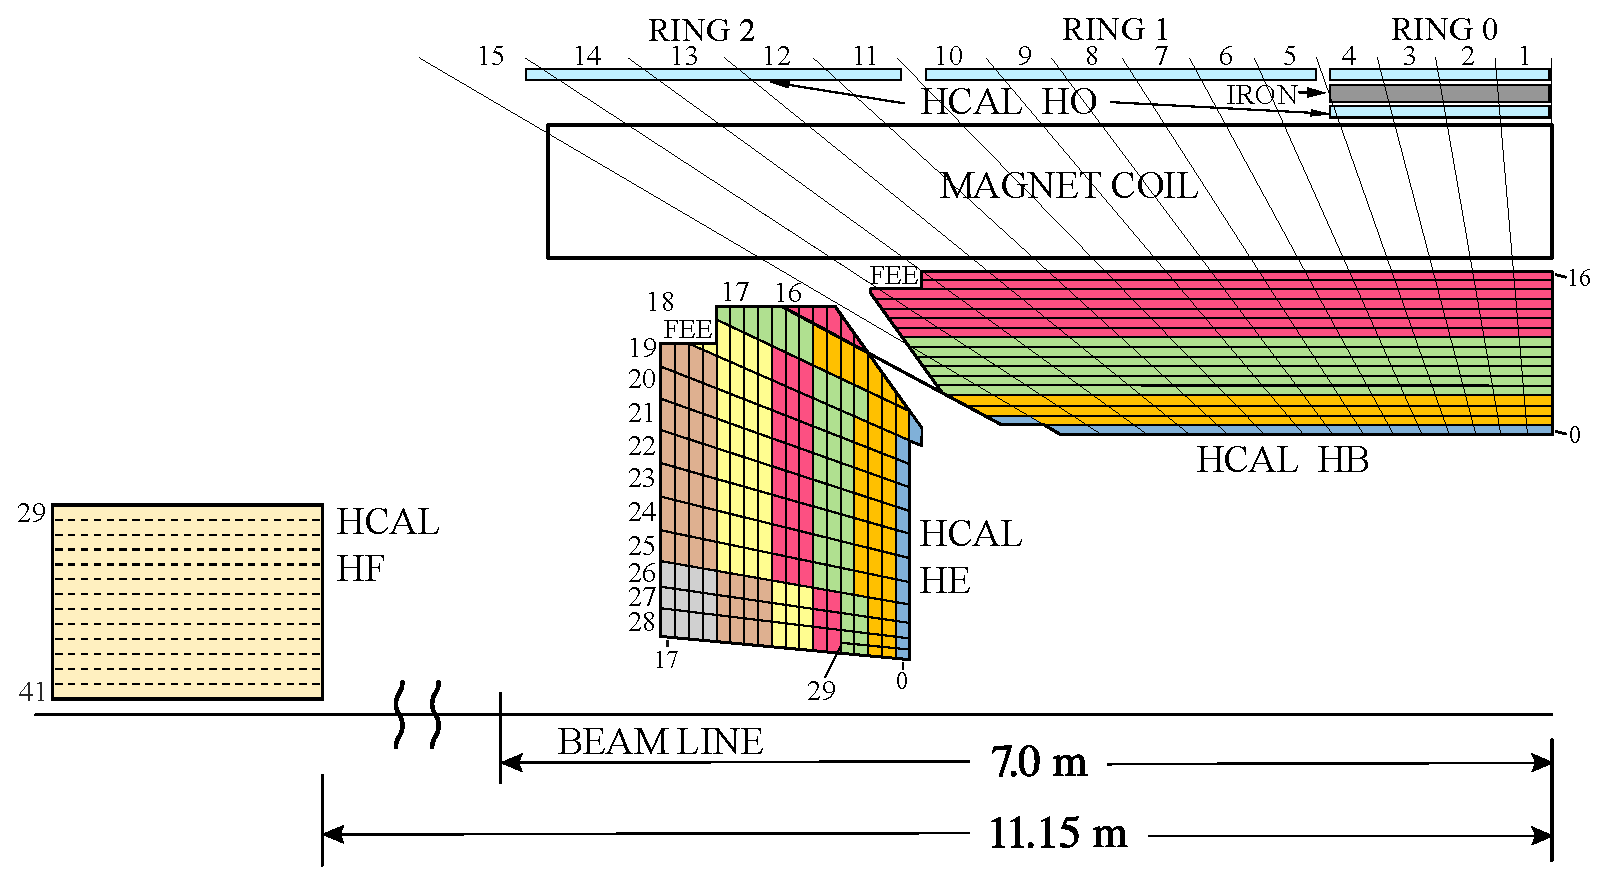
\includegraphics[width=0.8\textwidth]{figures/c3/c3_cms_2dhcal.pdf}
 \end{center}
 \caption{Phase 1 HCAL tower segmentation in the r,z plane.}
 \label{fig:c3cms2dhcal}
\end{figure}

The HB and HE are the major components of the HCAL. They are typical sampling calorimeters with brass from recycled Russian naval shell casings and scintillator for ~ 70000 tiles. Lights from the scintillators is collected and amplified by hybrid photodiodes (HPDs) in the phase 0 HCAL. The HPDs will be replaced with Silicon photomultipliers (SiPMs) for Phase 1 because the SiPMs are less noisy and more stable in heavy radiated area. 

After the photon detectors, the analog signal is delivered to the FrontEnd electronics. The charge pulse is integrated and digitized on the charge integrator and encoder (QIE). In the phase 1 upgrade, we will replace the QIE8 with QIE11 for all frontend readout modules in HE. The QIE11 have a much better time resolution, which is on the level of 0.5 ns. 

After the FrontEnd, the digitalized signal is delivered from the commission cavern to the service cavern through a long bonded fibers bundle. The backend electronics located in the service cavern receives those signals, generates the trigger primitives and delivers the signals to the central DAQ link. The HCAL backend electronics were upgraded from VME to uTCA on HB and HE during the 2015-2016 year-end technical stop (YETS)~\cite{CMS:2012tda}. 

However, due to the limitations of the ``compact" cavern, the EB and HB cannot provide complete containment for the hadronic showers. The HO is inserted just between the solenoid and muon system to ensure adequate sampling depth in the barrel region. The solenoid coil is used as the absorber for HO, which measures the shower deposit after HB. 

The HO detector construction is the same as the phase 0 HB and HE, except for the photon detectors. The HO has the SiPMs instead of HPDs since the LHC long shut down 1. The SiPMs have proved to be very reliable in the current operation except for a small leakage current drift monitoring issue at the beginning of LHC Run 2. 

The last component of HCAL is the Forward calorimeter (HF). The calorimeter design is severely challenged by the extremely high radiation environment. Therefore, quartz fibers are used as the active medium for HF. When a shower occurs, Cherenkov light is emitted in the quartz fiber and transported to photomultiplier tubes (PMT). The HF also provides input to the CMS luminosity measurement. 

In summary, there are four subdetectors in HCAL: HB, HE, HO and HF. There are 9216 readout channels for HB, 6912 for HE, 2376 for HO and 3456 for HF in the HCAL phase 1 scheme. The backend electronics coordinates are compressed into the RAW event data after the event builder in the HLT. On one hand, the offline reconstruction software and online data quality monitor need to know the detector geometry coordinates in order to map the digitalized output into physical space. We need to build a database object to map the backend coordinates and detector coordinates. On the other hand, the backend electronics are not connected directly to the HCAL tiles: we still have photomultiplier and frontend electronics in between. HCAL has several different upgrade projects for different parts of different sub detectors during the LHC Run 2. Therefore, we need a dynamic map, which reflects the real connections among all HCAL components. This map is called the HCAL logical Map. The logical map starts with frontend coordinates, maps upwards to the photomultipliers, and then detector tiles, and downwards to the backend coordinates and trigger primitive channels. We avoid re-designing everything after the each upgrade with this dynamic structure of the map. 

To build a robust HCAL logical map, we need inputs from experts in different fields. For example, we need to follow a special symmetric design in the frontend to backend optical patch. This symmetry is highly dependent on the firmware design. Although nowadays FPGA (Field Programmable Gate Array) can be programmed with less restriction, we still need to keep the algorithm maintainable. We also plot the backend and detector coordinates respectively in frontend coordinates in order to check the symmetry in the mapping (Fig~\ref{fig:c3cmshcalhelmapfebe} and Fig~\ref{fig:c3cmshcalhelmapfegeo}).

\begin{figure}[htbp]
 \begin{center}
  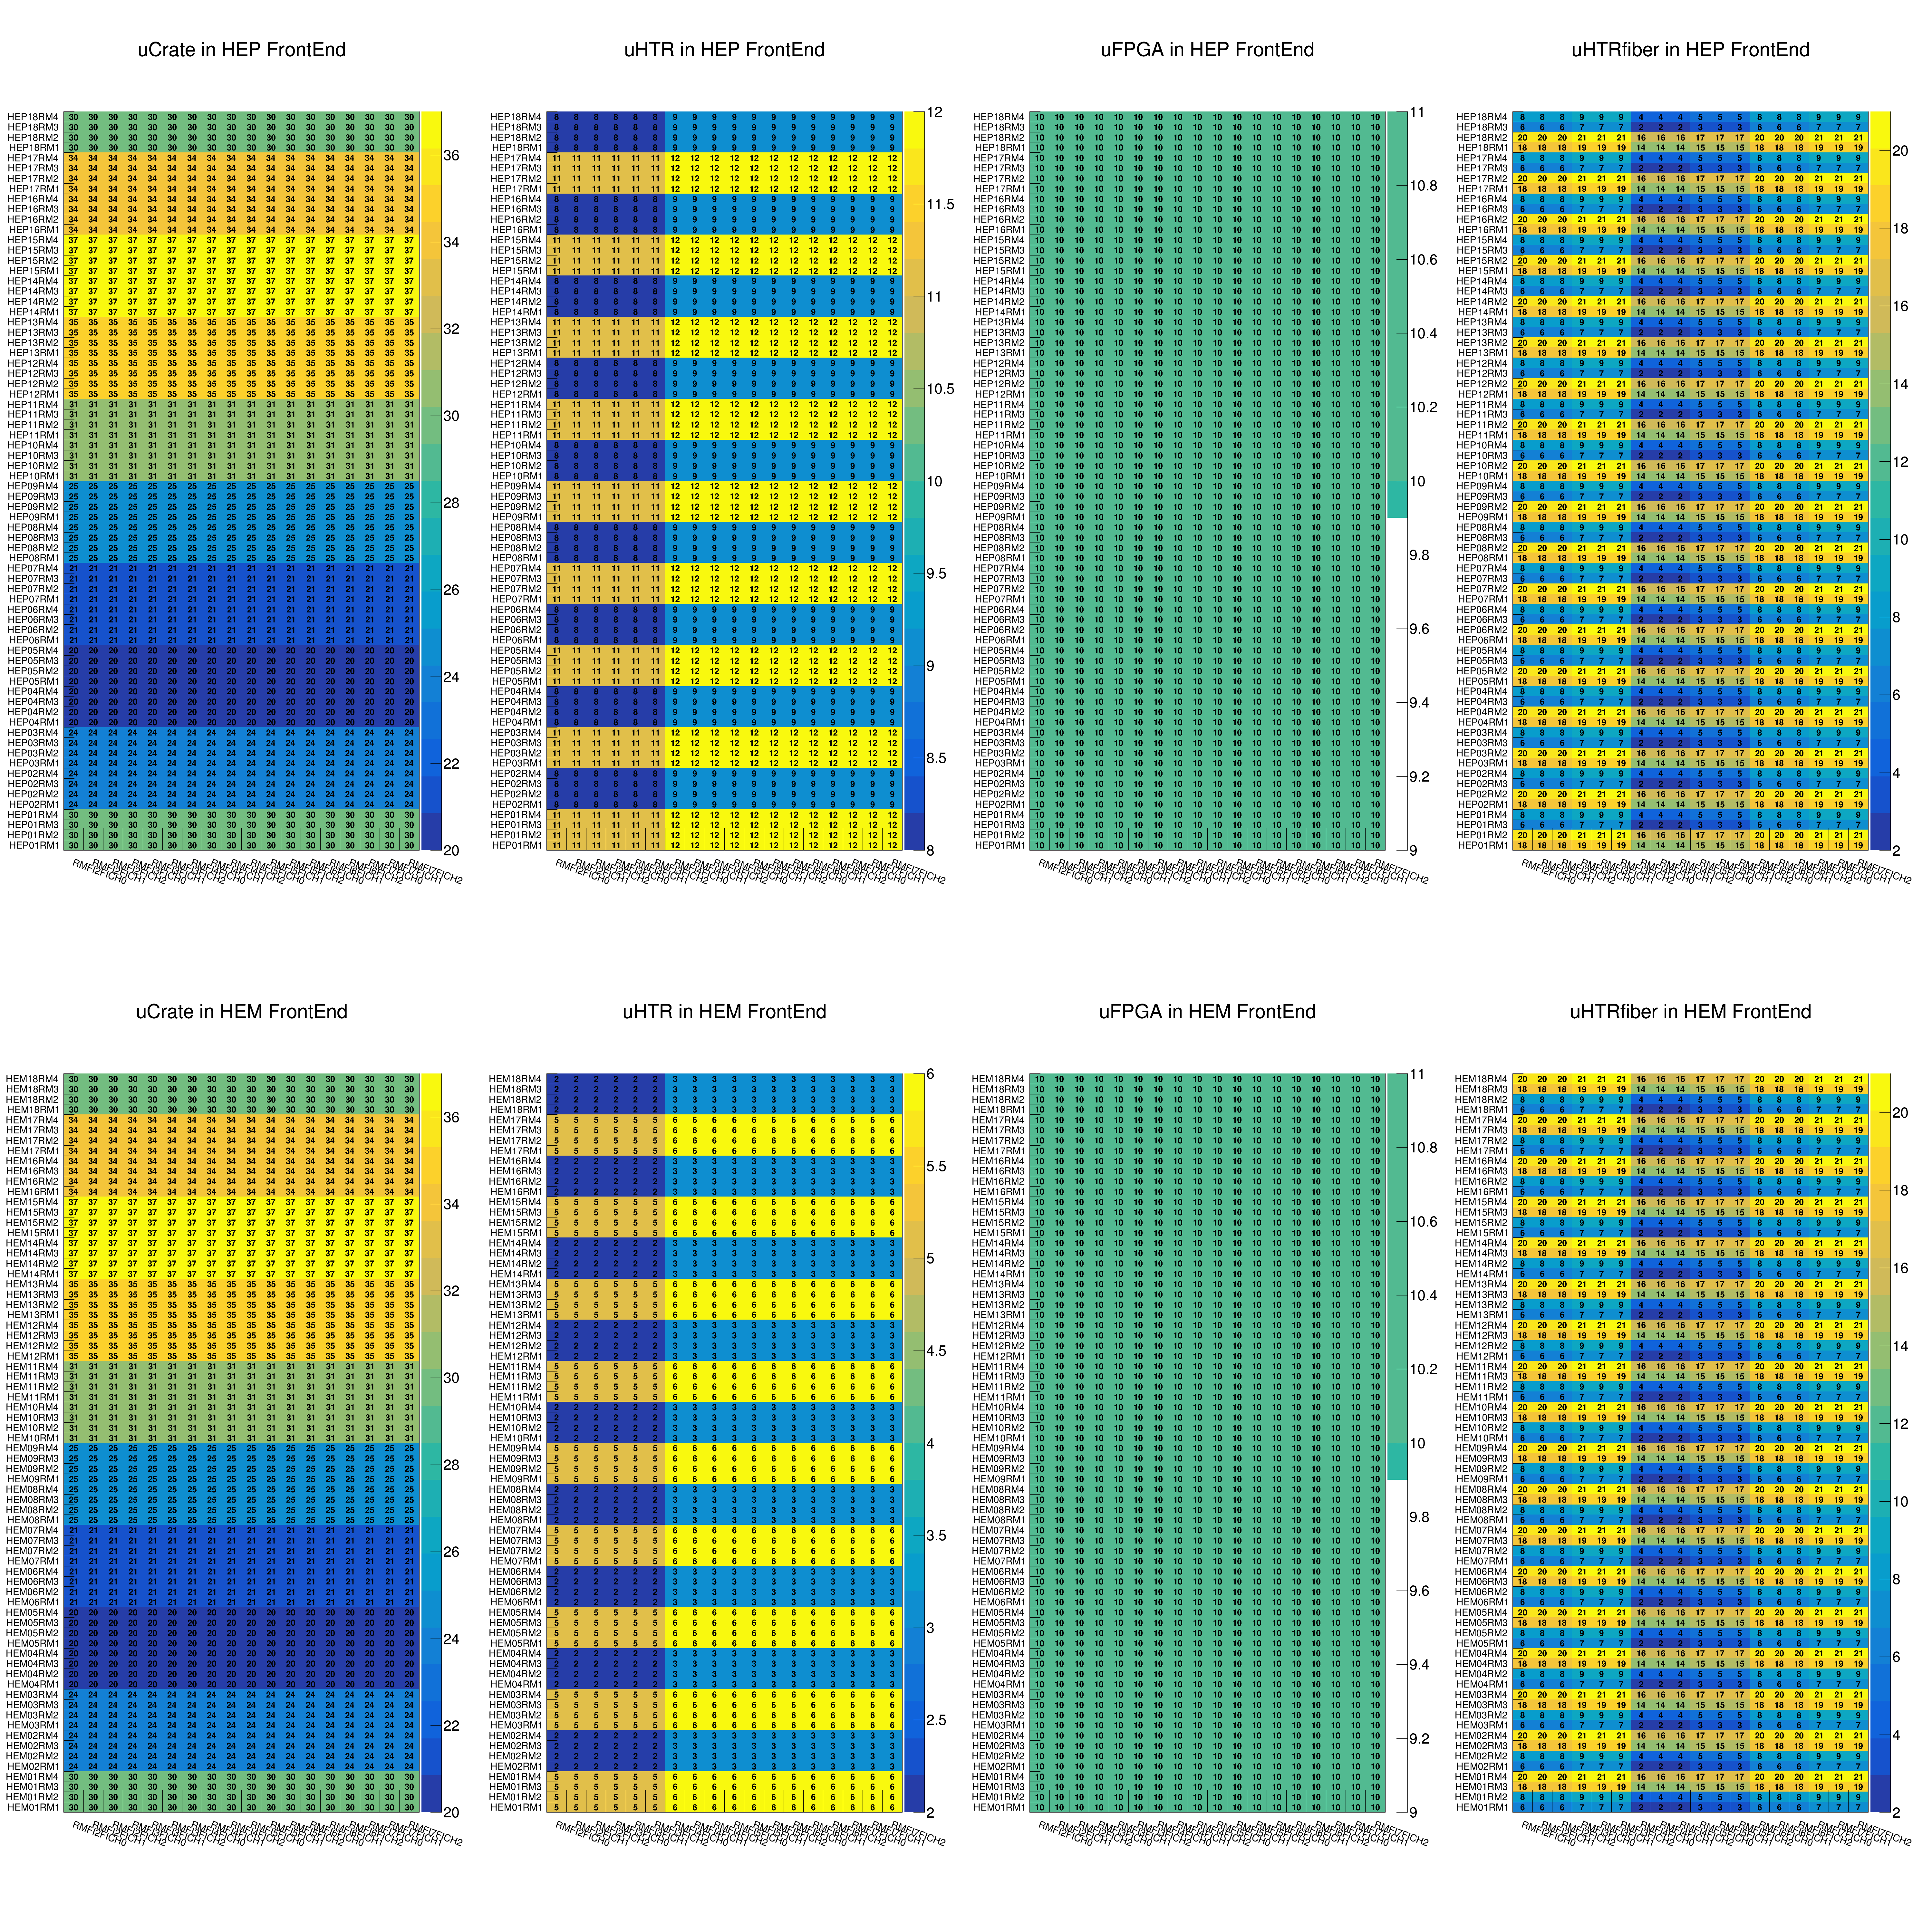
\includegraphics[width=0.8\textwidth]{figures/c3/c3_cms_hcalhelmapfebe.png}
 \end{center}
 \caption{Backend coordinates in Frontend coordinates, HCAL endcap phase 1 backend plus phase 0 frontend in 2016 operation.}
 \label{fig:c3cmshcalhelmapfebe}
\end{figure}

\begin{figure}[htbp]
 \begin{center}
  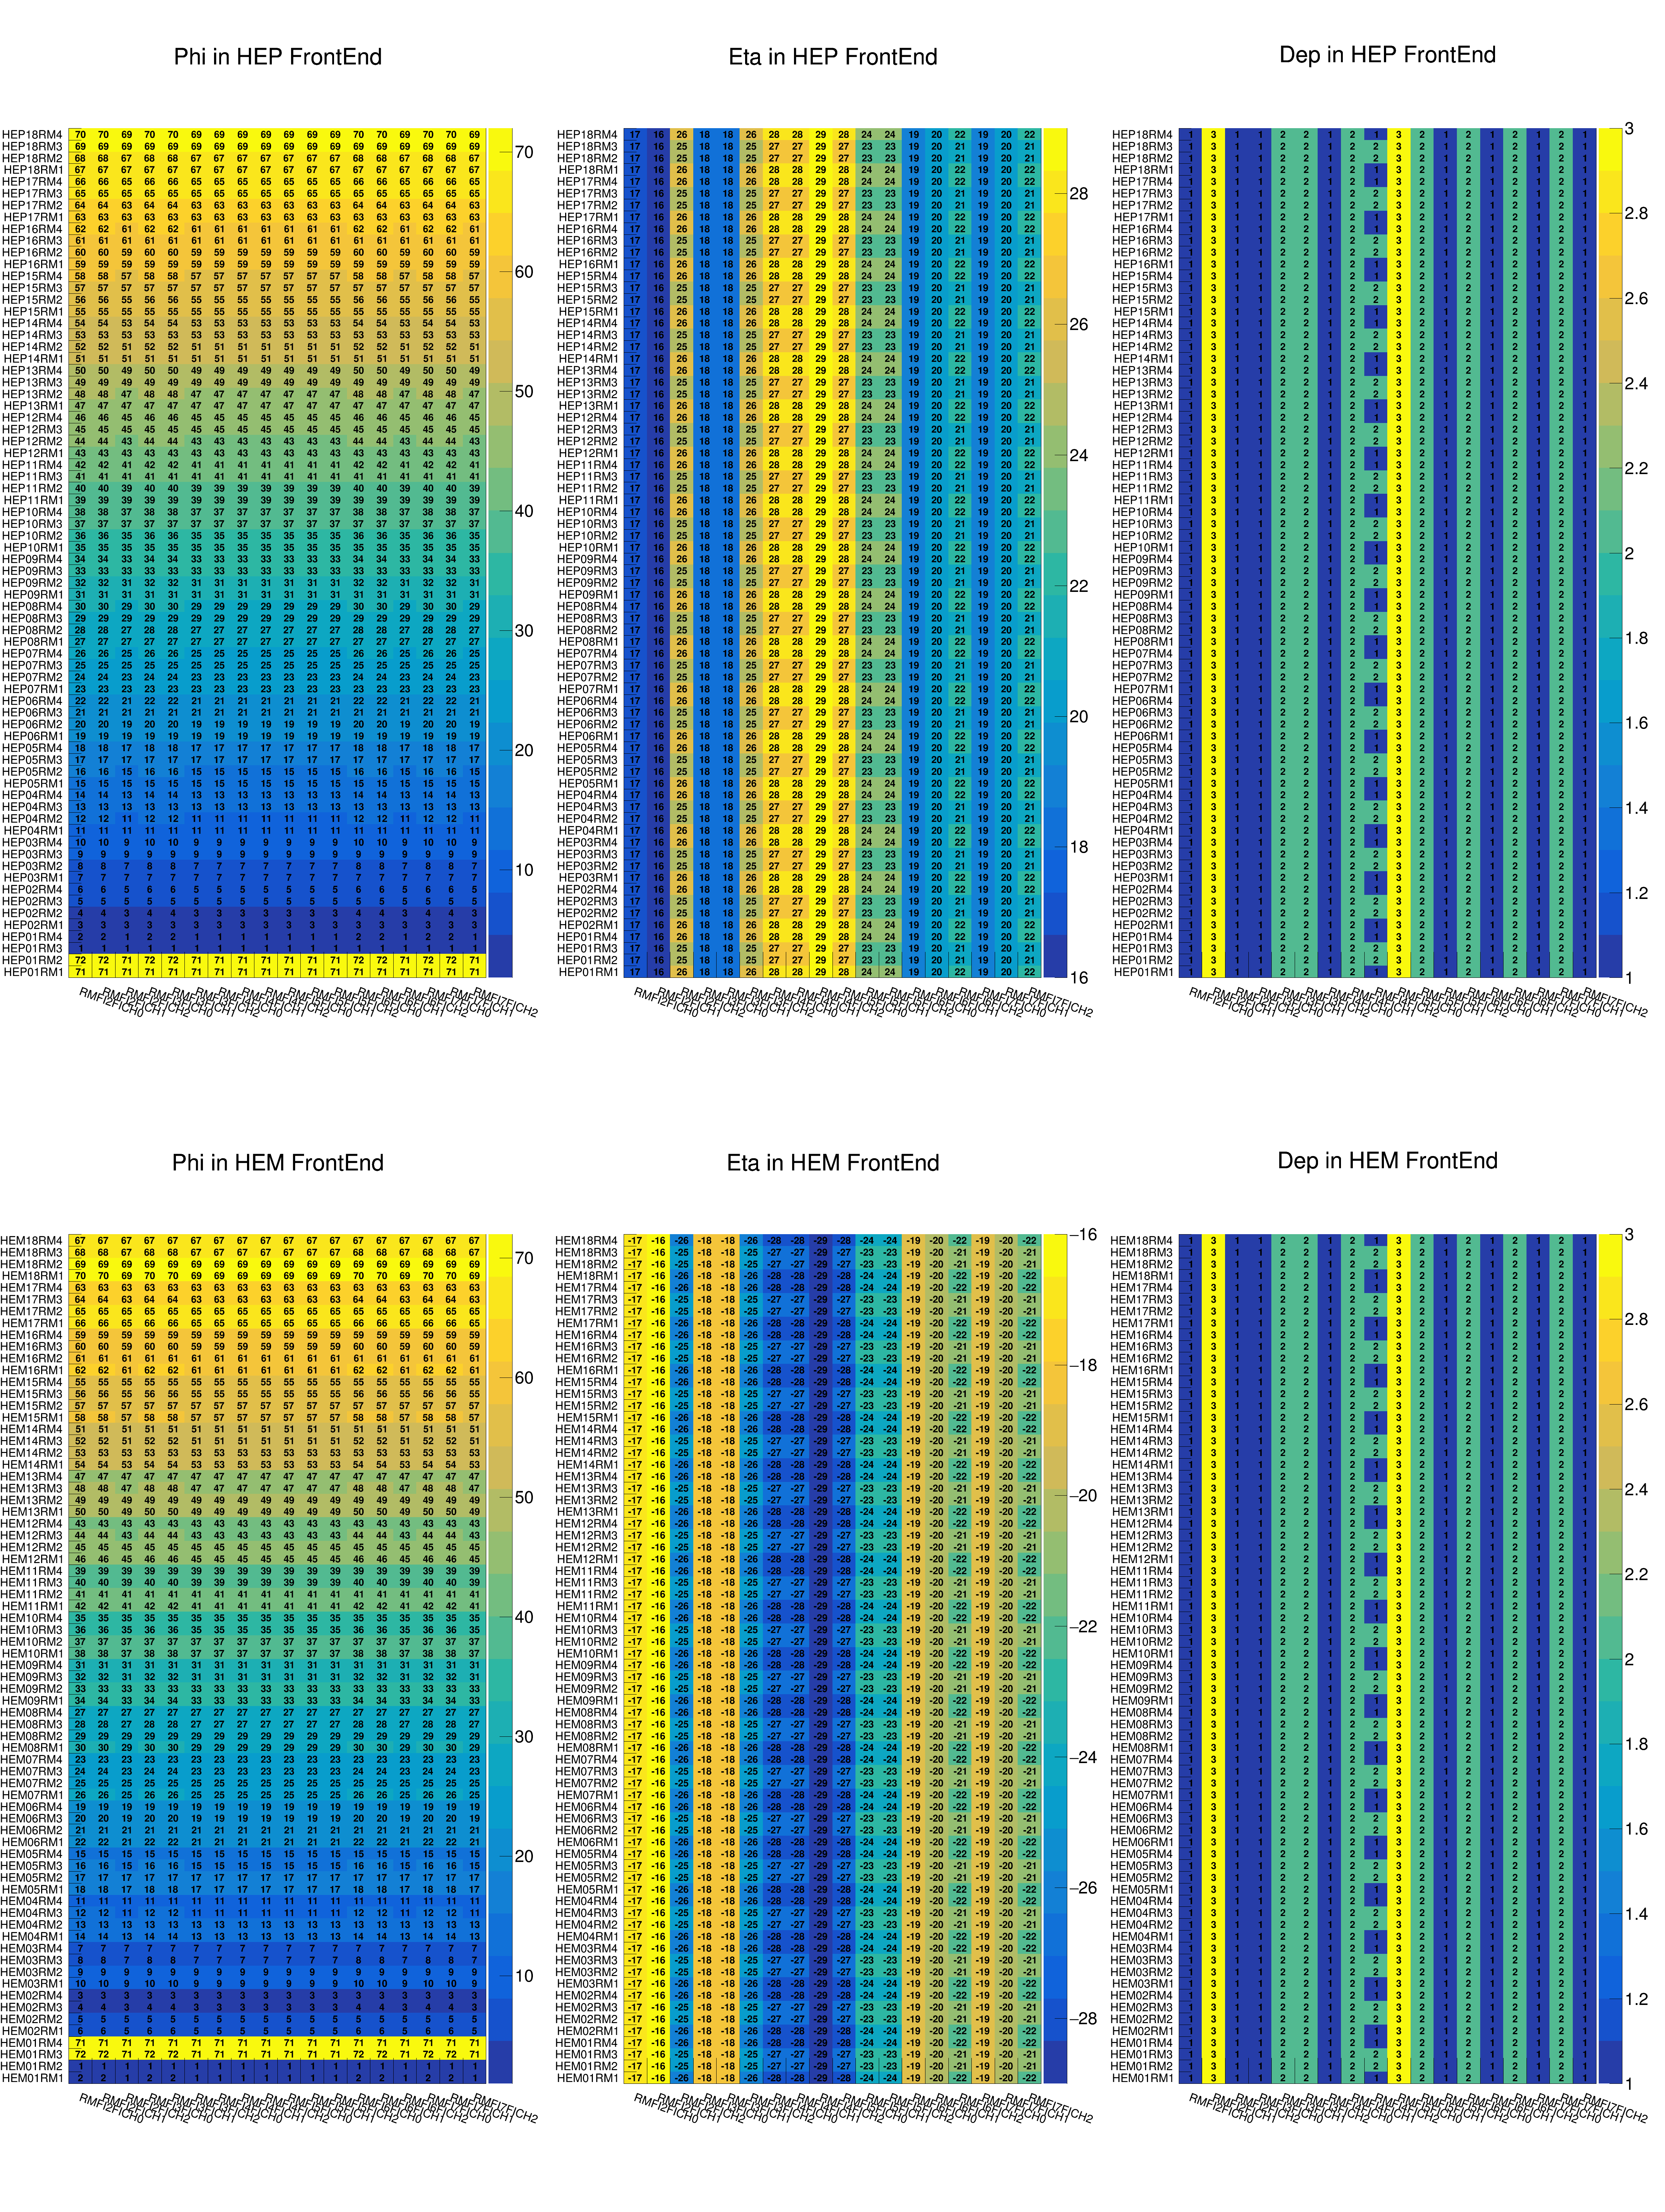
\includegraphics[width=0.8\textwidth]{figures/c3/c3_cms_hcalhelmapfegeo.png}
 \end{center}
 \caption{Detector coordinates in Frontend coordinates, HCAL endcap phase 1 backend plus phase 0 frontend in 2016 operation.}
 \label{fig:c3cmshcalhelmapfegeo}
\end{figure}


Subsets of the HCAL logical map are critical in the HCAL software. One of the most important applications is the electronics map (EMap). The HCAL electronics map is a subset of the logical map that contains backend coordinates and detector coordinates. As was mentioned, the reconstruction software needs the EMap database to obtain the detector coordinates from the backend coordinates. This is a necessary step in the RAW to DIGI reconstruction and in the DIGI to RAW conversion in MC simulation. Another application is the QIE calibration table. In the DIGI to RECO step, we need to translate from ADC (Analog Digital count) to the fC with the piecewise linear QIE gain function. This map is produced from the logical map. The robustness of the logical map is critical for the HCAL offline reconstruction. 

\subsubsection{Muon detectors}

The importance of the muon detectors is implied by the experiment’s middle name (``M" in CMS). The CMS muon detectors provide measurements of muon track coordinates. The measurement of muons is important in both in standard model physics (e.g. Higgs to ZZ) and in new physics searches (e.g. searches for supersymmetric particles that can decay to leptons). Moreover, the muon system provides a muon-related level-1 trigger that is used to reduce the data rate.

The CMS muon detectors consist of three sub-detectors: Drift tubes in the barrel region, cathode strip chambers in the endcap and resistive plate chambers in both the barrel and endcap. A layout of CMS muon detectors is shown in Fig~\ref{fig:c3cms2dmuondets}. More details are given in the following sections. 

\begin{figure}[htbp]
 \begin{center}
  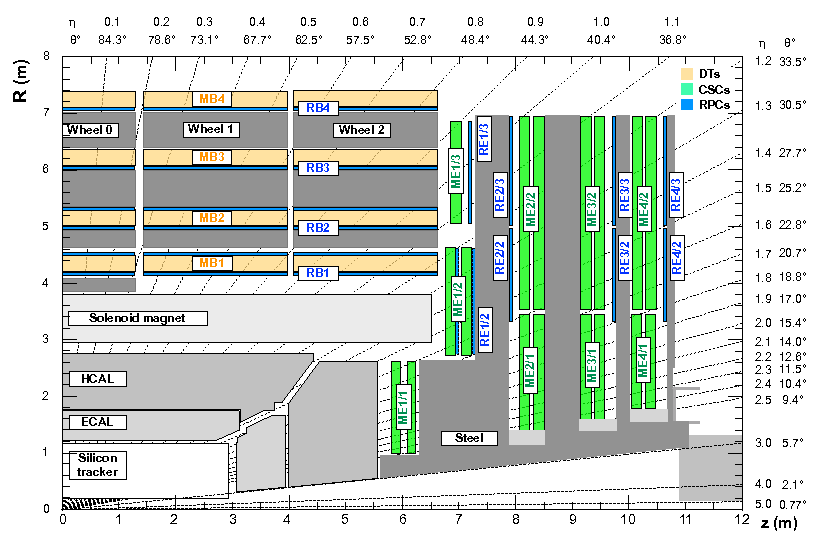
\includegraphics[width=0.8\textwidth]{figures/c3/c3_cms_2dmuondets.png}
 \end{center}
 \caption{Two dimensional CMS inner tracking system layout, phase 0.}
 \label{fig:c3cms2dmuondets}
\end{figure}

\paragraph{Drift tubes}
The drift tubes (DT) are the part of CMS muon detectors that measure the muon tracks in the barrel region. The basic unit of the drift tubes is the drift cell. A drift cell is a 42mm-wide tube containing a thin conductive wire at high positive voltage within a gas volume. The muon knocks electrons off the atom of the gas when it traverses the chamber. The muon tracks can be reconstructed by measuring the drift time for different cells. 

Like the HCAL outer detector, the drift tubes contain 5 wheels along the z-axis, 4 stations for each wheel, labeled MB1, MB2, MB3 and MB4. The three inner stations have 60 drift chambers each and the outer chamber has 70. A drift chamber consists of 2 or 3 super layers, each made of by 4 layers of drift cells staggered by half a cell. This honeycomb geometry gives an excellent time-tagging capability, with a time resolution of a few nanoseconds. The full DT provides a pseudo-rapidity coverage of $0<|\eta|<1.2$.

\paragraph{Cathode strip chambers}
The cathode strip chambers (CSC) are the CMS muon detectors located in the endcap region. The CSC is also a type of wire chamber, but differently from the DT, the CSC measures the location (to be specific, phi coordinates) instead of drift time. The CSC consists of arrays of positively charged anode wires crossed with negatively charged copper cathode strip within a gas volume. The muon knocks electrons off from the gas atom. Then electrons move to the anode wire to create an avalanche. Positive ions also move to the cathode and trigger a charged pulse.

The CMS endcap muon system consists of 468 cathode strip chambers in the following arrangement: 72 ME1/1, 72 ME1/2, 72 ME1/3, 36 ME2/1, 72 ME2/2, 36 ME3/1, 72 ME3/2, and 36 ME4/1. The full CSC provides a pseudo-rapidity coverage of $1.2<|\eta|<2.4$. 

The RPC is designed as a fast response provider for the trigger. However, for the endcap region, the CSCs by themselves are sufficient for the trigger requirements for the current instantaneous luminosity of the LHC. Moreover, the CSCs have a better spatial resolution and a larger pseudo-rapidity coverage, providing better precision for the measurements of endcap muons.

\paragraph{Resistive plate chambers}
Resistive plate chambers (RPC) are fast gaseous detectors that provide a muon trigger system in parallel with the DT and CSC. The RPC consists of a two high resistively plastic parallel plates with gas between them. One of the plates is a positively charged anode and the other is a negatively charged cathode. Like the CSC, electrons of the gas molecules will be knocked off when a muon passes through, and trigger an avalanche. The pattern of hits from the cathodes provides a quick measurement of the muon momentum, which is sent to the trigger for decision-making. In the CMS RPC, the double-gap modules are used instead of the single-gap modules. This allows a lower bias voltage for each single-gap and higher detector efficiency. The RPC has both good spatial resolution and time resolution (one nanosecond). 

The CMS RPCs are distributed in both the barrel and endcap regions. There are 96 RPCs in each wheel in the barrel region. More details on the distribution are given in Table~\ref{tab:c3cmsrpc}. In the endcap region, there are 3 RPC stations in the phase 0 design. In order to retain high muon reconstruction efficiency with Run 2 condition, a fourth disk was installed during the long shutdown 1 as part of the phase 1 upgrade. The full RPC has the same pseudorapidity coverage as the DT in barrel, and a smaller coverage ($1.2<|\eta|<2.1$) than the CSC in the endcap.

\begin{table}[htbp]
\fontsize{10 pt}{1.2 em}
\selectfont
\begin{centering}
\caption{\label{tab:c3cmsrpc} Numbers of RPCs for different wheels.}
\hspace*{-4ex}
\begin{tabular}{|c|c|c|c|c|c|c|}
\hline
 RPC &  W+2 & W+1 & W0 & W-1 & W-2 & Total \\
\hline
 RB1(in) & 12 & 12 & 12 & 12 & 12 & 60 \\
\hline
 RB1(out) & 12 & 12 & 12 & 12 & 12 & 60 \\
\hline
 RB2/2(in) & 12 & - & - & - & 12 & 24 \\
\hline
 RB2/2(out) & - & 12 & 12 & 12 & - & 36 \\
\hline
 RB2/3(in) & - & 12 & 12 & 12 & - & 36 \\
\hline
 RB2/3(out) & 12 & - & - & - & 12 & 24 \\
\hline
 RB3 & 24 & 24 & 24 & 24 & 24 & 120 \\
\hline
 RB4 & 24 & 24 & 24 & 24 & 24 & 120 \\
\hline
 Total & 96 & 96 & 96 & 96 & 96 & 480 \\
\hline
\end{tabular}
\par\end{centering}
\end{table}

\subsubsection{Trigger system}

The LHC has a bunch crossing every 25 ns, which means an intrinsic data rate of 40 MHz. It is impossible for the data acquisition and storage system to deal with such a high rate, and it is not necessary either, since not all the events are interesting for physics analysis. Therefore, we need a system to reduce the data rate and select the events that we are interested in. The system is called trigger system --- only triggered data will be read and stored from the LHC collision. 

The CMS trigger system is a 2-level trigger system: the FPGA based L1T (Level 1 trigger) and PCs farm based HLT (High level trigger). In the old days (e.g. Tevatron, CDF trigger) there was a custom hardware L2T layer between the L1T and HLT to ease the computing speed gap. However, with improvement to the computing power of the PCs farms, we can avoid the additional L2T. This gives a more robust system with a less complicated structure. 

The CMS L1T system receives part of its information from the sub detectors and performs a rough reconstruction of physics object at the FPGA level. The data rate is reduced from 40 MHz to 100 kHz (85 kHz to 90 kHZ in real operation, mainly limited by the data acquisition system) after the L1T. The CMS L1T was upgraded (Phase 1) during the 2015-2016 YETS and 2016-2017 EYETS to account for the large increase in the LHC beam intensity in Run 2. The scheme for the phase 1 L1T is shown in Fig~\ref{fig:c3cmsl1scheme}. The calorimeters send the trigger primitive to the calo trigger layer from where the signals are sent to the global trigger. The muon system sends information to the global muon trigger from where they are sent to the global trigger. The L1A (level 1 acceptance) is generated and sent to the sub detectors through TCDS (timing, control and distribution system). The sub detectors send the information to the data acquisition or keep on taking data for next bunch crossing based on the L1 decision. 

\begin{figure}[htbp]
 \begin{center}
  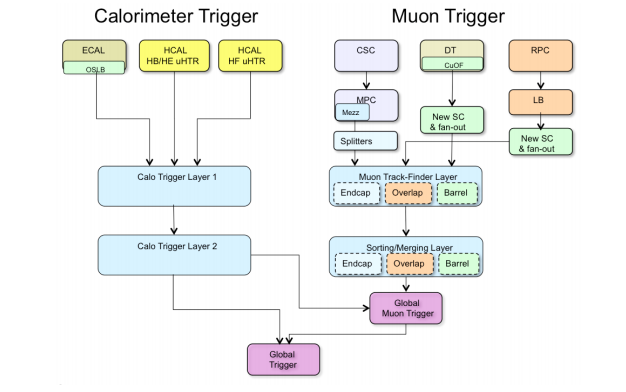
\includegraphics[width=0.8\textwidth]{figures/c3/c3_cms_l1scheme.png}
 \end{center}
 \caption{Dataflow for the overall phase 1 trigger system.}
 \label{fig:c3cmsl1scheme}
\end{figure}

The CMS HLT system uses all the information from the detector readout and applies a simplified algorithm to reconstruct physics objects. Promptly reconstructed objects are used in the high-level trigger menu for various physics purposes. However, just like the L1T, the HLT has bandwidth limitations. The data rate after the HLT is around 1000 Hz which is limited mainly by offline storage rather than online computing. HLT is the interface between physics analysis and online operation. On one side, each physics analysis group has a trigger contact person to collect the desired trigger menu from analyzers and make a proposal for a full menu set with rate estimation to the HLT that satisfies the data rate limit. On the other side, each HLT menu takes at least one L1 seed as a starting point of the high-level trigger.

The current (Phase 1) trigger system will continue in operation until the end of LHC Run 3. However, there will be a huge challenge on the trigger system with the HL-LHC. The Track trigger will be necessary to maintain the current physics acceptance with the L1 rate around 1 MHz. 

%\clearpage
\subsection{Event reconstruction}

The data from the central data acquisition system is selected and built in the high-level trigger farm and then transferred to the primary computing grid at CERN (Tier-0). The data directly from the detector electronics is called DAQ-RAW, which is the input of the online HLT cluster. The data is reformatted and filtered with the high-level trigger. The outcome data are called RAW. Compared to the DAQ-RAW, the RAW contains the HLT information and is ready for offline reconstruction after reformatting. 

Before entering the offline reconstruction chain, the data stream is filtered into different primary datasets (PD) for various purposes. Most of the categories are based on physics analysis and the level 1 trigger. For example, in the all-hadronic SUSY search, the common PD for the search region is HTMHT or MET. For the control region, we can select SingleElectron or SingleMuon PD. Then, the RAW with different PD streams is delivered into the offline reconstruction system (CERN Tier-0 or any Tier-1, Fig~\ref{fig:c3cmstiers}). 

\begin{figure}[htbp]
 \begin{center}
  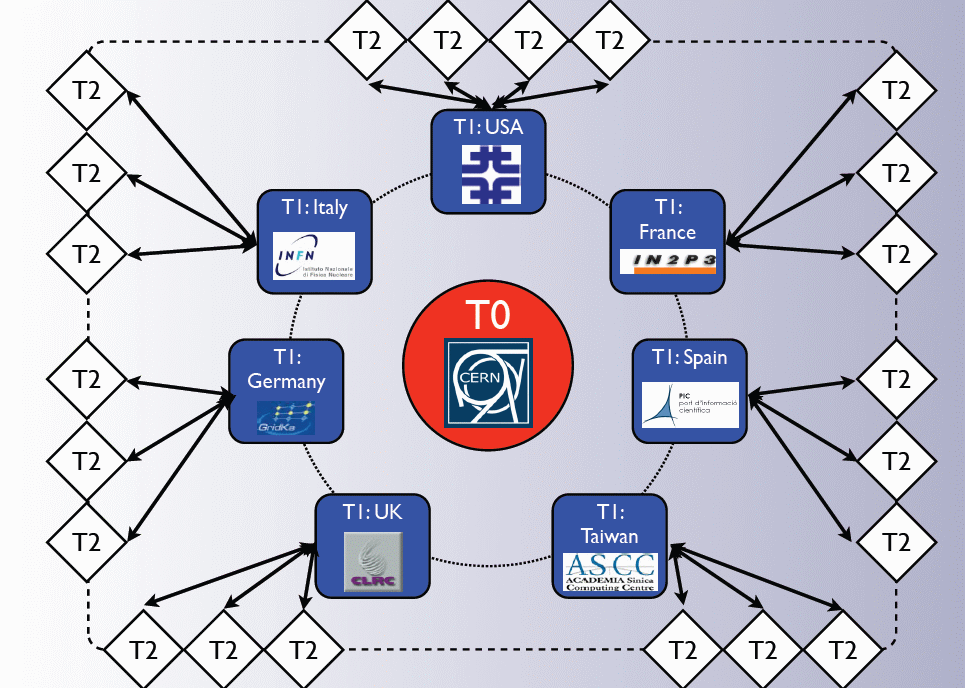
\includegraphics[width=0.8\textwidth]{figures/c3/c3_cms_tiers.png}
 \end{center}
 \caption{CMS offline computing structure.}
 \label{fig:c3cmstiers}
\end{figure}

In the offline reconstruction, the RAW dataset is unpacked from the electronics based digital counts to detector based digital hits. This is the so-called RAW to DIGI step in the reconstruction. After that, the DIGI is converted to reconstructed hits with calibration information. This is called DIGI to RecHits step. The offline database is highly involved in these 2 steps, providing the electronic-detector map, calibration table, pedestal subtraction, radiation damage correction, etc. Then, the physics objects are generated with the reconstruction algorithm. The dataset after the offline reconstruction is called RECO, which combines the RecHits and physics object information together. 

However, the size of the RECO dataset is about 1.3 MB per event. Further reduction of the event size is necessary for the physics analyses. Therefore, information that is not commonly used for physics analysis is dropped to form a new data format: miniAOD (AOD stands for Analysis Objects Data). It contains the standard physics objects used by most CMS physics analysis groups. More details on those objects are discussed in the following sections. 

\subsubsection{Tracks}

Tracks are detected by inner silicon detector signals and form the basis of the event reconstruction. Track reconstruction serves the following purposes: 
\begin{itemize}
\item Vertex reconstruction: The vertexes in proton-proton collisions can be reconstructed from the intersecting point of tracks. However, there can be multiple vertexes in an event because the pile up effect. 

%Run 1
%The vertex with the maximum sum of the square of the $p_{T}$ of all the associated tracks is identified as the primary vertex. 
The reconstructed vertex with the largest value of summed physics-object $p_{T}^2$ is taken to be the primary proton-proton interaction vertex. The physics objects are the objects returned by a jet finding algorithm~\cite{Cacciari:2008gp,Cacciari:2011ma} applied to all charged tracks associated with the vertex, plus the corresponding associated missing transverse momentum.

We also reconstruct secondary vertices, i.e., vertices displaced from the beam line, which can indicate the positions of the decay of long-lived particles. Secondary vertex information is very important for b-jet identification.
\item Momentum measurement: The CMS inner silicon system has a high resolution in the track momentum measurement thanks to the strong magnetic field (3.8 T). The jet $p_{T}$ measurement benefits from the high precision track momentum with the particle flow algorithm. More details are covered in the jet reconstruction section.
\item Particle identification: Charged particles can be identified with track information. For example, an electron candidate is found when the energy deposit in the ECAL supercluster can be associated with a track. Muon identification is performed by matching a track from the inner detector with a track segment from the muon detector.
\end{itemize}

Given the importance of track reconstruction in physics, a reliable algorithm is required. The desirable algorithm must have a near 100\% efficiency in track reconstruction together with a relatively small fake rate. The jet energy can be badly mis-measured if there is an unreconstructed or fake track.
There are two steps in the track reconstruction: 
\begin{itemize}
\item Local reconstruction: the signals from the strip and pixel are clustered to evaluate the position and error matrices of hits.
\item Global reconstruction: Tracks are reconstructed with several iterations of the combinatorial track finding method~\cite{Adam:2005cg}. Different seeds are used in different iterations to improve the tracking efficiency for various types of tracks.
\end{itemize}
The track finding algorithm is very powerful. It can even find tracks with very low energy ($p_{T}<2~GeV$). Some of the low energy tracks have more hits than the number of detector layers because they spiral in the magnetic field. Other tracks do not reach the preshower detector. Those tracks are kept in the data file for low energy physics studies at CMS. 

\subsubsection{Electrons}
Electron reconstruction in CMS relies on the information from the inner tracker and ECAL. The track momentum can be measured with smaller uncertainty in the inner tracker system. On the other hand, the calorimeter has a better resolution for high-energy objects. Therefore, a mixture of ``ECAL seed" and ``tracker seed" algorithms is designed to optimize the electron identification in both the high and low $p_{T}$ spectrum. 

The ECAL seed electron identification algorithm starts from the supercluster energy deposit in the ECAL. The supercluster is a 5 by 5 cluster combination of lead tungstate crystals in the ECAL. The initial energy and position of the supercluster are used to estimate the electron trajectory in the first tracker layer. In contrast, the tracker-based method begins with the tracks reconstructed by the general algorithm for charged particles. The tracks filtered using a pre-selection criteria and then matched to an ECAL supercluster. This mixture of seed method has been validated with electrons from W boson decays in 2010~\cite{Khachatryan:2015hwa}. 

The electron identification group provides several working points to satisfy the needs of various physics analysis groups. For example, we choose the ``Veto" working point in the SUSY analysis described in this thesis. The ``Veto" has the loosest identification criteria, which helps us to reject background events containing electrons to the maximum extent. 
\subsubsection{Jets and particle flow}

A jet is a collimated flux of stable hadrons that originates from a quark or a gluon following hadronization. A jet algorithm is a method to reconstruct the jets. There are several different jet algorithm approaches, but the inputs of the jet algorithm are always the clustered energy deposits in 2-dimensional plane. 

There are two major requirements for a jet algorithm: that it be collinear safe and infrared safe. Collinear safe means that the results of the jet algorithm are invariant under collinear splitting of any input momentum. Infrared safe means that a soft emission does not change the results of jet algorithm. Infrared safe is required not only from soft QCD emissions, but also from the collider point of view: the jet algorithm results should not change because of a soft jets from pile-up. 

The anti-$k_{T}$ algorithm~\cite{Cacciari:2008gp} is the standard jet algorithm at the LHC. The anti-$k_{T}$ algorithm is a sequential recombination algorithm. In this approach, we define a special distance between two input observables as in  Eq~\ref{eq:c3cmsantikt}:

\begin{equation}
 d_{ij} = min(k_{Ti}^{-2},k_{Tj}^{-2})\frac{(\eta_{i}-\eta_{j})^{2}+(\phi_{i}-\phi_{j})^{2}}{R^{2}}, \;
 \label{eq:c3cmsantikt}
\end{equation}
where $k_{Ti}$ is the transverse momentum (or any other response) of the ith input. The numerator is the geometrical distance between the two objects. R is the cone size parameter in the algorithm. The CMS experiment supports R=0.4 for the normal jets and R=0.8 for fat jets. Fat jets are useful in the analysis of highly boosted objects, as will be described in top tagging section below. The special distance between an input object with respect to the beam direction is defined as: $d_{iB} = k_{Ti}^{-2}$.

The first step is to compute all the $d_{ij}$ and $d_{iB}$, and find the smallest one. Then the following steps are iterated until all objects are clustered into a jet: 

\begin{itemize}
  \item If the smallest one is a $d_{ij}$, we combine the two objects i and j, remove objects i and j from the list of objects, and add the combined entity to the list of objects, calculating its $d_{ij}$ and $d_{iB}$. The combined object is given by the sum of the four-momentum of objects i and j.
  \item If the smallest one is a $d_{iB}$, we remove object i and call it a jet.
\end{itemize}

The anti-$k_{T}$ algorithm is both collinear and infrared safe. The geometrical distance between two collinear objects is zero. Therefore these two objects will be clustered first. The special distance is infinite for a soft object whose transverse momentum approaches zero. Therefore this new object will be clustered last, contributing nothing to the jet it is associated with since its transverse momentum is zero, or will form a new jet with zero transverse momentum. The jet results for the anti-$k_{T}$ algorithm remain unchanged in either case. 

There are other algorithms that are also both collinear and infrared safe, like the SiSCone~\cite{Salam:2007xv} and $k_{T}$~\cite{Cacciari:2005hq} algorithms. However, unlike these latter two algorithms, jets from anti-$k_{T}$ algorithm always have a nearly circular jet area~\cite{Cacciari:2008gn}, which makes them easier to correct for detector-related effects.

The performance of jet finding in CMS is improved using the particle-flow (PF) algorithm~\cite{CMS-PAS-PFT-09-001} and by using PF candidates as the input to the anti-$k_{T}$ jet clustering. 

The particle flow algorithm is a particle reconstruction and identification method that uses the information from all sub detectors. The PF algorithm is especially important for CMS jet and missing transverse momentum reconstruction because of the uncompensated nature of the CMS HCAL. A jet usually has three components from: charged hadrons ($\pi^{+},\pi^{-}$, etc.), photons ($\pi^{0}$), and neutral hadrons ($K_{L}$, etc.). The typical fractions of the three components are listed in the Table~\ref{tab:c3cmsjetf}. The inner tracker can provide a precise measurement of the charged hadron fraction. The CMS ECAL provides an excellent measurement of the photon energy. The remaining 10\% of the jet energy, due to the neutral hadron fraction will not give a huge uncertainty to the final measurement, on average. 

\begin{table}[htbp]
\fontsize{10 pt}{1.2 em}
\selectfont
\begin{centering}
\caption{\label{tab:c3cmsjetf} Average Jet components in GEANT4 Simulation.}
\hspace*{-4ex}
\begin{tabular}{|c|c|c|c|}
\hline
Jet Constituent & Energy Fraction & Detection Instrument & Uncertainty \\
\hline
Charged Hadron  & 65\% & Inner Tracker & Negligible \\
\hline
Photon          & 25\% & ECAL &  $0.07^{2}E_{jet}$ \\
\hline
Neutral Hadron  & 10\% & ECAL and HCAL & $0.16^{2}E_{jet}$ \\
\hline
\end{tabular}
\par\end{centering}
\end{table}

The key aspect of the PF algorithm is the linking of charged particles between the tracker and calorimeter. First, a track collection is generated, using the iterative track reconstruction method that described in previous section. Then, energy deposits in the calorimeter are clustered to obtain an initial identification of photons, charged hadrons, and neutral hadrons. A linking algorithm~\cite{CMS-PAS-PFT-09-001} is applied to connect the objects from the inner tracker and calorimeters. 

The PF jets are still not the collection that is directly used in the physics analyses. The PF jet energies still need to be corrected. For the data, there are three corrections that are applied. The first correction accounts for pile-up and noise. This correction is related to collider and detector effects and is subtracted from the raw energy. The second correction accounts for reconstruction effects, and is evaluated using MC simulation. Finally, the jet energy is corrected with di-jet data. More details of the jet energy corrections are given in~\cite{1748-0221-6-11-P11002}. The jet energy corrections are applied in both data and MC in the physics analysis described in this thesis. 

\subsubsection{Missing transverse momentum}

The missing transverse momentum (\MET) is the imbalance in the transverse momentum in an event, and is calculated as the negative of the vector sum of all objects in the event. The \MET is an important variable in supersymmetry searches that assume R-parity since the LSP is assumed to escape without detection, leading to potentially significant \MET. The \MET is a powerful variable to suppress the standard model background in the search region. 

However, on the reconstruction side, \MET is a high-level variable since all visible particles are used in its calculation. Unexpected effects from the detectors or collider issues in object reconstruction can give us the wrong \MET. Therefore, we need to establish robust \MET filters before we use the \MET, especially for the high \MET case. Source of abnormal \MET can be HCAL noise in the HPDs, beam halo, etc. 

After the filters, \MET needs to be corrected, similarly to the jet energies. The usual way to do this in CMS is to propagate the jet energy correction to \MET (so-called Type 1 correction). We apply the type 1 correction in this analysis. More details on the \MET filters and corrections are covered in Ref.~\cite{CMS-PAS-JME-16-004}. 


\subsubsection{Muons}
Muons are particles that can penetrate the calorimeter. They are detected when they traverse the muon detectors, outside the solenoid. Muon reconstruction is based on several approaches: 

\begin{itemize}
	\item Global Muon reconstruction: The muon tracks are reconstructed first inside the muon system (DT, RPC, CSC) with a standalone method. Then, the muon-system standalone track is matched with a tracker track by comparing the parameters of the two tracks. Finally, a global muon track is derived by fitting the hits of the two tracks using the Kalman-filter method~\cite{Fruhwirth:1987fm}. This is so-called outside-in method since we start from the muon system, which is outermost element of the CMS detector. 
  \item Tracker Muon reconstruction: This approach begins with the track reconstructed in the inner silicon detectors. Tracks with $p_{T}<0.5~GeV$ and momentum $p>2.5~GeV$ are selected as the potential muon candidate. Then, the track is extrapolated to the muon system considering the magnet field, average expected energy loss and multiple coulomb scattering effects. The track is considered to be a muon track if at least one muon hit is matched with this track. This is called inside-out method since it begins with the inner tracker system. 
\end{itemize}

The global muon reconstruction method has a better momentum resolution for high $p_{T}$ muons. The reason is that the inner tracker system covers only a small radial distance, limiting its ability to accurately measure the $p_{T}$ of high $p_{T}$ tracks, which exhibit little curvature in the magnetic field. However, the tracker muon reconstruction method has a better performance for soft muons. This originates from the excellent low $p_{T}$ track reconstruction provided by the inner tracker system. 

A particle-flow based algorithm has been designed to provide good performance for both soft and hard muons. This particle flow muon reconstruction method is a combination of the outside-in and inside-out methods. In this approach, global muon tracks and tracker tracks are gathered together and then selected with special criteria. The selection criteria are adjusted depending on environment of the muon (e.g. isolation) and other detector inputs (e.g. energy deposit in calorimeter). This method is optimized to identify muons within jets. The performances of the three approaches have been studied in Ref.~\cite{Chatrchyan:2012xi}. 

%\clearpage
\subsection{Event simulation}
Event simulation is critical in particle physics analysis. The simulation of the CMS experiment can be categorized into two parts: physics process simulation and detector performance simulation. The former one is the proton-proton collision physics and the latter one is the detector response simulation. 

The simulated events are also called MC (Monte Carlo). Monte Carlo is the name of a famous casino house in Monaco. High-energy physicists use MC as a reference to the random numbers in the event-generation processes. This jargon will be used in this thesis. 

\subsubsection{Physics process simulation}

The physics process simulation is described in this section. The high-energy proton-proton process calculation is based on the QCD factorization theorem~\cite{Collins:1989gx}. The QCD factorization theorem declares that the hard-scattering cross section is a convolution product of a parton distribution function and a perturbative calculable hard scattering. Therefore, the non-perturbative aspects of QCD are incorporated into the parton distribution function. To summarize, the differential cross section of a proton-proton collision can be expressed by Eq~\ref{eq:c3cmsppdf}:

\begin{equation}
 %\begin{aligned}
  \begin{split}
		\frac{\sigma_{pp \rightarrow X}}{d\Phi}=& \sum_{\{s_{i}\}} \int \prod_{i} \frac{d^{3}q_{i}}{(2\pi^{3})2E_{i}} \sum_{ab} \int dx_{a}dx_{b}(2\pi)^{4}\delta^{4}(x_{a}p+x_{b}p\prime-\sum_{i}q_{i}) \\
	                                          & f_{a}^{PDF}(x_{a})f_{b}^{PDF}(x_{b}) \frac{1}{2\hat{s}}|M|^{2}(ab \rightarrow \{s_{i}\};x_{a},x_{b},\{q_{i}\}) D(X(\{x_{i},q_{i}\};\Phi)), 
  \end{split}
 %\end{aligned}
 \label{eq:c3cmsppdf}
\end{equation}
where M is the matrix element, a calculable quantity in perturbative QCD and $f^{PDF}$ is the parton distribution function (PDF)~\cite{Butterworth:2015oua}. The PDF cannot be calculated from first principles. Therefore, the PDF needs to be parameterized and determined from data. There are several different PDF collaborations, e.g. CTEQ~\cite{Lai:2010nw} or NNPDF~\cite{Ball:2014uwa}. In Run 2, CMS uses the CTEQ6L1 PDF set. The D is the fragmentation function, which states the probability for the outgoing parton $s_{i}$ to produce the final state X through the hadronization process. The fragmentation function, like the PDFs, cannot be derived from first principles but must be determined from data.

In practice, it is not practical to calculate the cross section directly from Eq~\ref{eq:c3cmsppdf} because there are too many combinations of final-state hadrons for the given outgoing partons. Therefore, the calculation is truncated before the hadronization stage and parton shower MC simulations are used to finish the calculation. Collinear parton splitting and soft gluon emission are considered at each order of the strong coupling strength in the parton shower simulations since they are dominant processes. Then the
partons from the shower are combined to form hadrons using models, such as the Lund string~\cite{Andersson:1983ia} or the cluster model, based on the preconfinement property of QCD~\cite{Amati:1979fg}. More details of the parton shower simulation are given in Ref.~\cite{Hoche:2014rga}.

Besides particles created in the hard scattering process, particles in proton-proton collisions can be created in soft processes, such as from the remnants of the protons left after the hard scattering of a quark or gluon from the protons has occurred. A schematic underlying process together with hard process event plot is shown in Fig~\ref{fig:c3cmsunderlyingevents}. We use minimum bias data collected using only very minimal trigger conditions to study the effects of underlying events. In the simulations, the properties of underlying events are tuned to describe the minimum bias data. More details are given in Ref.~\cite{Field:1393621}. 

\begin{figure}[htbp]
 \begin{center}
  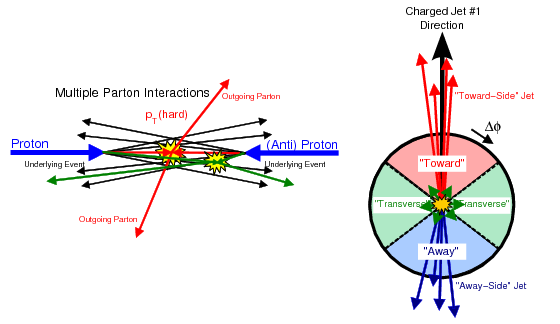
\includegraphics[width=0.8\textwidth]{figures/c3/c3_cms_underlyingevents.png}
 \end{center}
 \caption{Left: Illustration of the underlying event modeled by PYTHIA, together with hard process. Right: Illustration of the correlations in the azimuthal angle relative to the direction of the leading charged jet.}
 \label{fig:c3cmsunderlyingevents}
\end{figure}

In CMS, two event generators are used to simulate physics events. First, a multi-purpose parton level generator (e.g. MadGraph~\cite{Alwall:2011uj}) is used to calculate the matrix elements, incorporating the PDF information. Second, the parton shower and hadronization is described using either PYTHIA~\cite{Sjostrand:2014zea} or HERWIG~\cite{Bellm:2015jjp}. All stable and intermediate particles are stored in the MC record for study. The stable particles are passed to detector simulation software. This latter stage is described in the next section. 

\subsubsection{Detector performance simulation}

The four-vectors of the final-state particles are processed through a program to simulate the detector response. All the particles and their secondary products from electromagnetic or hadronic showers are traced and simulated from first principle in the full simulation. 

The core software for this simulation is GEANT4~\cite{Agostinelli:2002hh}, which is a software toolkit that simulates the passage of particles through matter. The detector geometry, in this case, the CMS detector geometry~\cite{Lefebure:1999wja} is the input to GEANT4. Each subdetector has a geometry input class. The corresponding general GEANT4 geometry class inherits this class. During the simulation, different particles will call various modules when they pass through the CMS detector system, depending on the type of subdetector. 

However, the CPU time required for the full simulation is huge due to the complicated CMS geometry and the nature of the first principle calculations. Therefore, CMS also has a fast simulation method~\cite{1742-6596-396-6-062016}. The aim of fast simulation is to reduce the CPU time but keep the event simulation quality at an acceptable level. The simplifications are applied in several parts. For example, the pile-up simulation is simplified, the tracker geometry is roughened, and the showers are simulated with an empirical formula rather than from first principles. The simulation process is greatly shortened because of these simplifications. 

The fast simulation method is used for SUSY signal events and for some standard model processes. We can use high level object, like jets, without concern with respect to accuracy in the fast-simulated samples. However, we need to be careful concerning higher-level information (e.g. quark-gluon likelihood) in those simplified samples since the geometry is simplified. For example, in this thesis, the customized top tagger needs a fast-full simulation scale factor before the limit setting, in order to correct for differences between the fast and full detector simulation. More discussion on this is given in the next chapter. 
